\section{E and B Power Spectra Slopes}

To probe the possible parameter space that gives rise to the observed EE and BB spectral
slopes reported by \citep{Planck18XI} we run our simulations through a range of
sonic $M_s$ and Alfven $M_a$ Mach numbers over the course of 12 separate
simulations at a resolution of $512^3$. Functionally this means that we have
simulations of varying initial magnetic field strengths $B_{rms}$ and rms gas
velocities $v_{rms}$ which may (and do) evolve throughout the course of the
simulation. We then plot the EE and BB power spectra and fit the slope within
the most likely inertial range (within the injection and dissapation scale).

\begin{figure}[h]
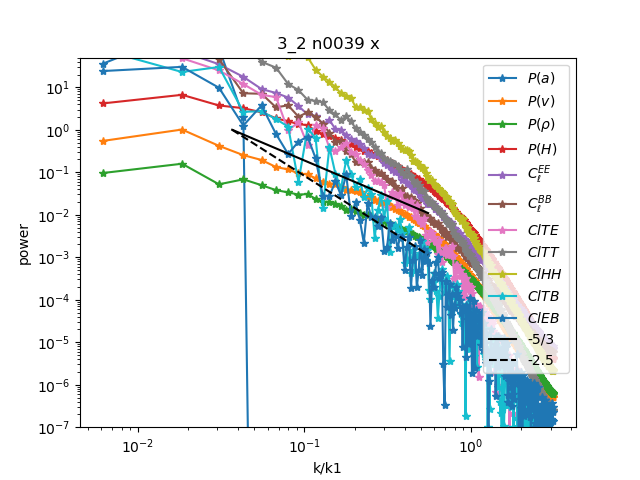
\includegraphics[width=\linewidth]{3_2_spectra_0039_x.png}
\caption{Example power spectra shown for various quantities at $M_s=3$ and
$M_a=2$ with line of sight along the magnetic field in a well evolved state
toward the end of the simulation run. Overplotted are the expected -2.5 slopes
for EE and BB observed by Planck et al. as well as the -5/3 slope which would be
observed for homogeneous self-similar Kolmogorov turbulence.}
\label{fig:example_spectra}
\end{figure}

In figure ~\ref{fig:example_spectra} we see a typical result for the observed
power spectra from various quantities in our simulation in a given run. In this
super-Alfvenic, super-sonic run we can observe the flatter left-most part of the
spectra corresponding to the injection scale, the relatively constant sloping
inertial range from which our measured slopes are drawn and the steeply sloped
dissapation scale toward the bottom-right of our spectra. 

\begin{figure}[h]
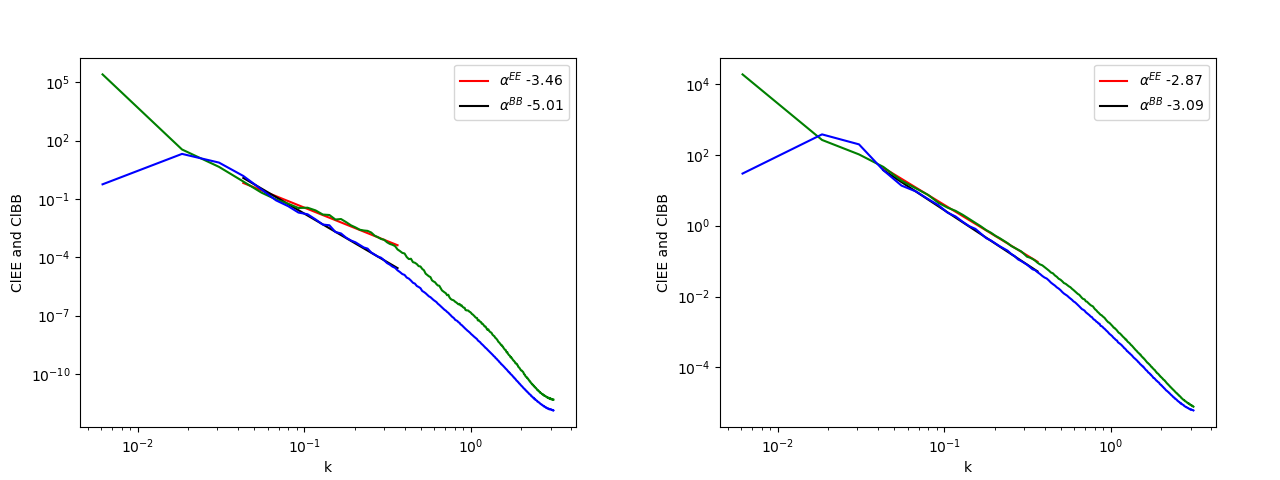
\includegraphics[width=\linewidth]{half_half_to_3_2_spectra_y.png}
\caption{Above we see how the EE (green line/red slope) and BB (blue line/black
slope) spectra change between a sub-sonic
($M_s=0.5$) sub-Alfvenic ($M_a=0.5$) (left-most image) and a super-sonic
($M_s=3$) super-Alfvenic ($M_a=2$) (right-most image) run.}
\label{fig:half_half_3_2_spectra}
\end{figure}

Looking specifically at the EE and BB power spectra we see in figure
~\ref{fig:half_half_3_2_spectra} generically that the spectra and their
respective slopes are largely influenced by the local values of $M_s$ and
$M_a$. Indeed the right-most image exhibits slopes much closer to the -2.5
values observed by the Planck collaboration. 

\begin{figure}[h]
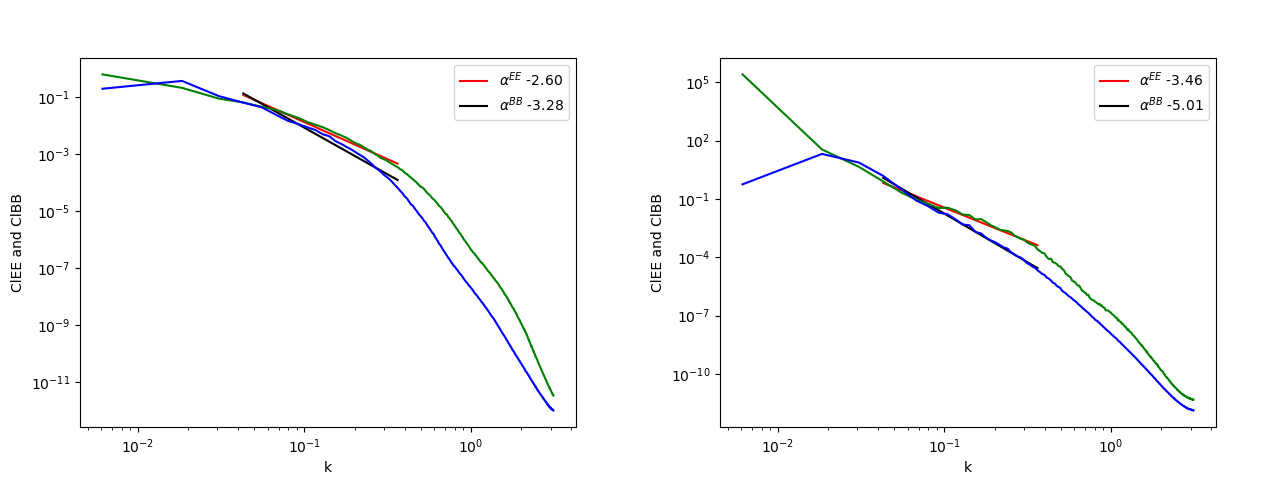
\includegraphics[width=\linewidth]{half_half_spectra_x_y.png}
\caption{The above figure shows how the EE (green line/red slope) and BB (blue line/black
slope) spectra can change for a given run between lines of sight. This sub-sonic
($M_s=0.5$) sub-Alfvenic ($M_a=0.5$) run image shows spectra observed with line of sight along the
background magnetic field (left-most image) and transverse to the field
(right-most image).}
\label{fig:half_half_los_spectra}
\end{figure}

Perhaps unsurprisingly we also find that the shape of the power spectra can be
strongly influenced by line of sight orientation relative to the direction of
the background magnetic field. This effect is most pronounced in the strong
field (low $M_a$) weak gas pressure (low $M_s$) runs where the magnetic pressure
dominates the flow. In figure ~\ref{fig:half_half_los_spectra} we can see two
very distinct EE and BB spectra taken from the same $M_s=0.5$ $M_a=0.5$
simulation run when looked at from lines of sight parallel (left image) and
transverse (right image) to the background magnetic field. When discussing the
results of our paramater space sampling on the observed slopes between runs we
must be careful to acknowledge the effect this has on the overall conclusions
drawn.

\begin{figure}[h]
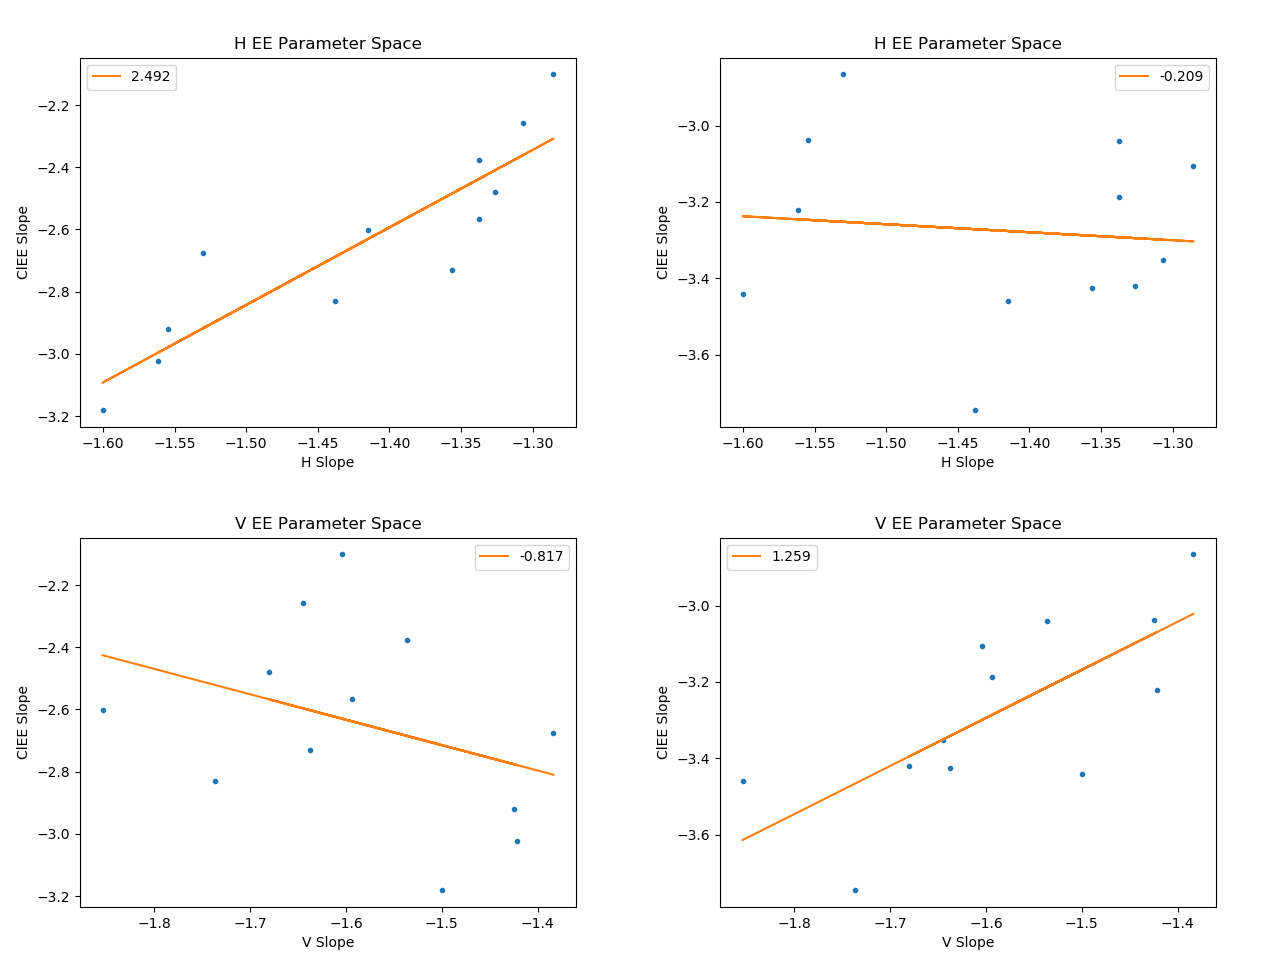
\includegraphics[width=\linewidth]{ee_V_H_x_y_paramspace.png}
\caption{Top Left: Slope of EE power spectra vs. slope of H-field spectra with
line of sight parallel to H-field. Top Right: Slope of EE power spectra vs. slope of H-field spectra with los transverse to H-field. Bottom Left: Slope of EE power spectra vs. slope of
velocity spectra with los parallel to H-field. Bottom Right: Slope of EE power spectra vs.
slope of velocity spectra with los transverse to H-field}
\label{fig:ee_V_H}
\end{figure}

\begin{figure}[h]
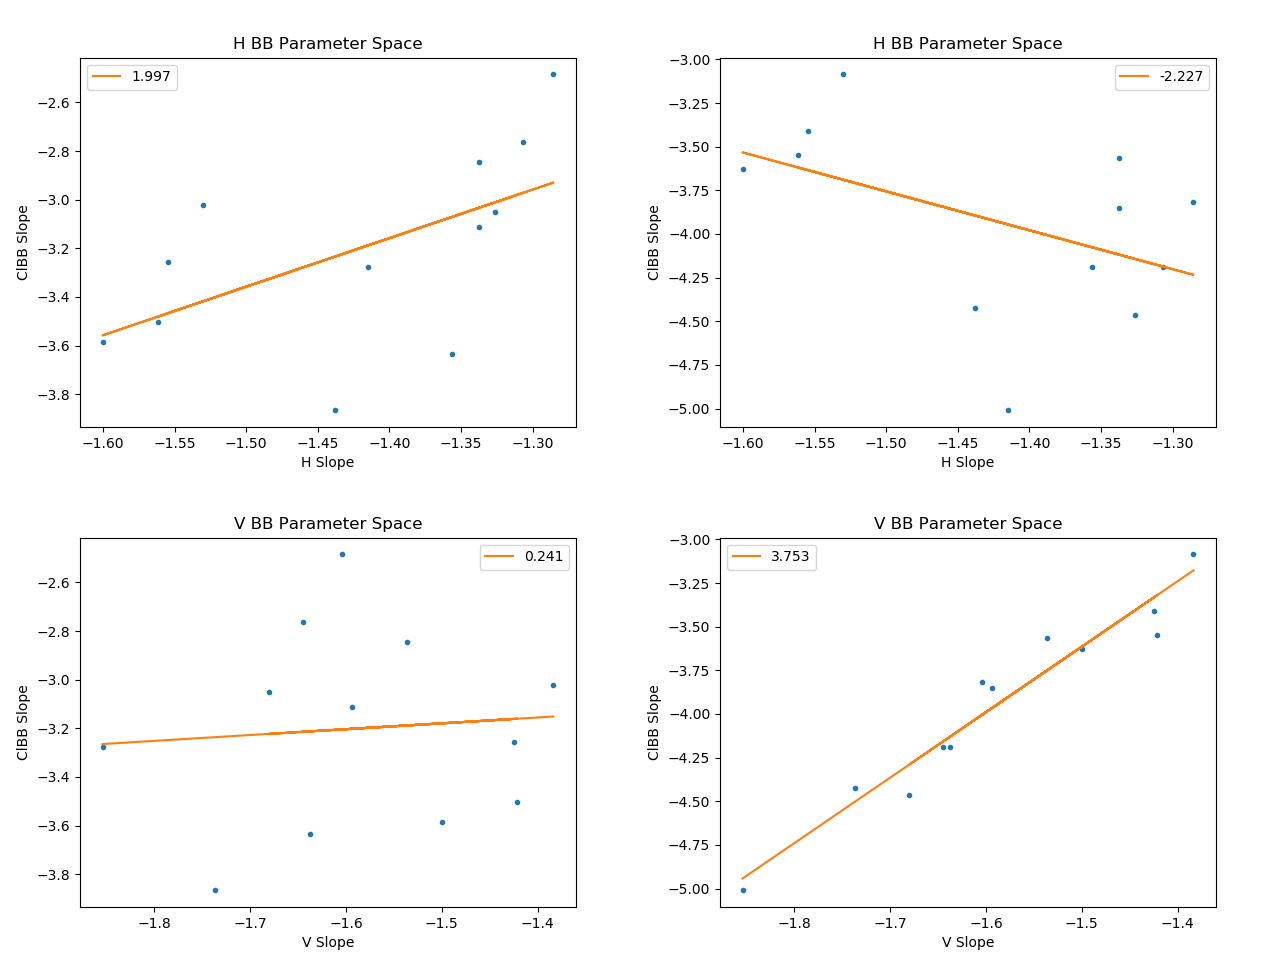
\includegraphics[width=\linewidth]{bb_V_H_x_y_paramspace.png}
\caption{Top Left: Slope of BB power spectra vs. slope of H-field spectra with
line of sight parallel to H-field. Top Right: Slope of BB power spectra vs.
slope of H-field spectra with los transverse to H-field. Bottom Left: Slope of
BB power spectra vs. slope of velocity spectra with los parallel to H-field.
Bottom Right: Slope of BB power spectra vs. slope of velocity spectra with los transverse to H-field}
\label{fig:bb_V_H}
\end{figure}

This line of sight effect on the power spectral slopes can be better understood
through figures ~\ref{fig:ee_V_H} and ~\ref{fig:bb_V_H}. These results clearly
demonstrate that for lines of sight along the magnetic field direction, the
shape of both the EE and BB spectra are closely correlated with the shape of
the magnetic field spectra and largely uncorrelated with the shape of the
velocity power spectra (left-most images in the figures). These figures also
demonstrate that the reverse is true when EE and BB are instead observed transverse to the magnetic field direction (right-most images in the figures).

\begin{figure}[h]
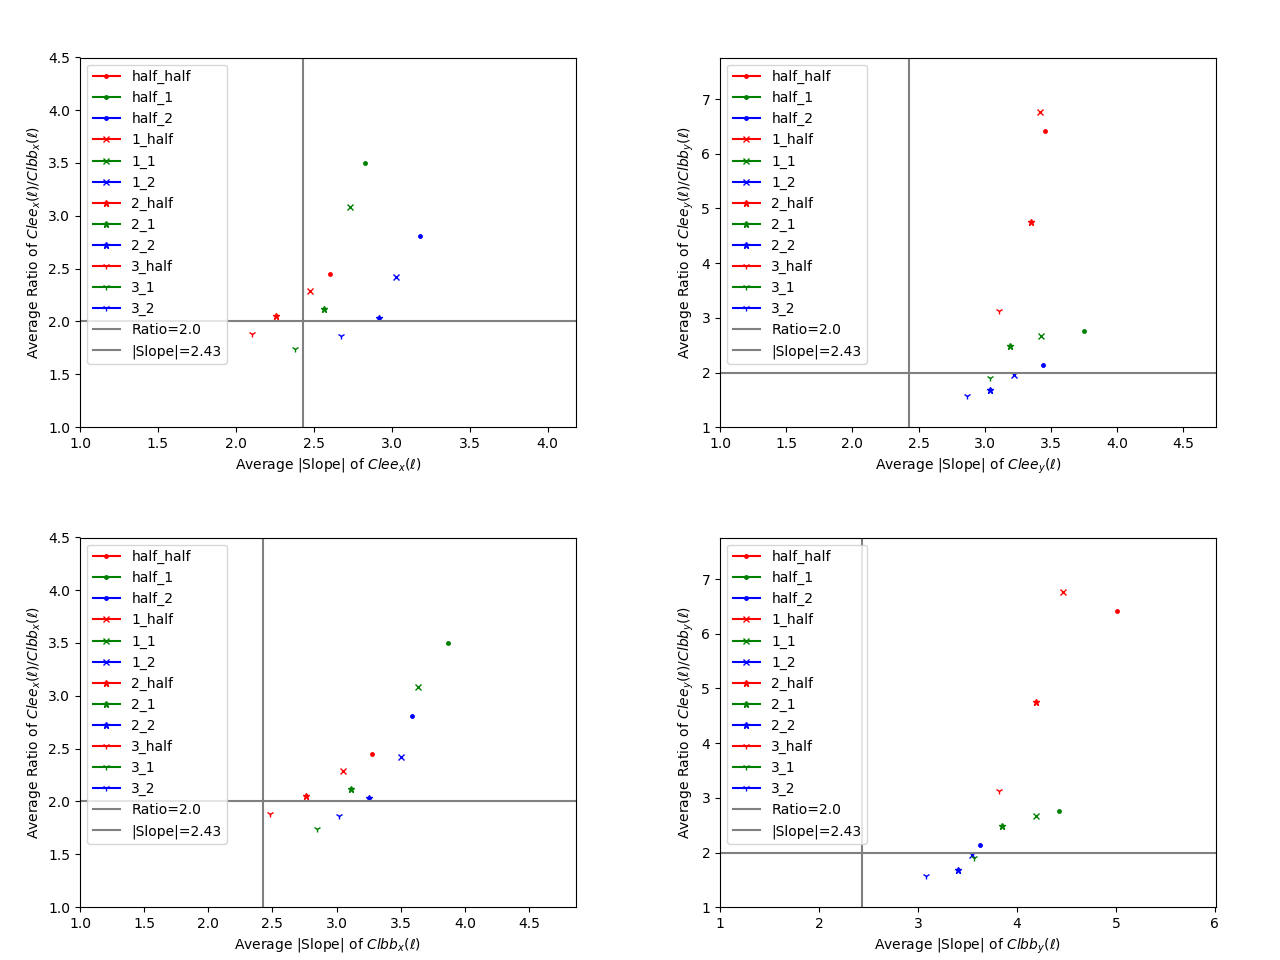
\includegraphics[width=\linewidth]{ee_x_y_bb_x_y_paramspace.png}
\caption{Top Left:Average E/B ratio $r$ vs Average EE slopes parallel to
magnetic field for all 12 simulations ran. Top Right: Average E/B ratio $r$ vs
Average EE slopes transverse to magnetic. Bottom Left: Average E/B ratio $r$ vs
Average BB slopes parallel to magnetic field. Bottom Right: Average E/B ratio
$r$ vs Average BB slopes transverse to magnetic field. All images have legends
labeled by $M_{s}\_ M_{a}$ associated with the simulation. Vertical and
horizontal grey lines in all images correspond to the $\alpha\approx-2.5$ and
$r\approx2$ respectively observed by \citep{Planck18XI}}
\label{fig:slopes_ratios_param}
\end{figure}

The main result of our survey and the overall effect that the above mentioned
correlations have on the observed slopes can be seen in figure
~\ref{fig:slopes_ratios_param} where we plot the observed EE and BB slopes
against their E/B ratios for all 12 of our various simulations. The horizontal
and vertical grey lines in the images represent the target E/B ratio
($r\approx2$) and target slope ($\alpha\approx-2.5$) respectively observed by
\citep{Planck18XI}.

With respect to $M_s$ and $M_a$ the slopes of EE and BB demonstrate two clear
properties. First for a given value of $M_a$, regardless of line of sight, both EE and BB have slopes that tend to become increasingly shallow as $M_s$ increases. This is
depicted in the figure by observing that for a given color ($M_a$), the order of
the symbols from left to right is the same in all cases and strictly decreasing
in sonic Mach number ($M_s$).

The second general observation on the spectral slopes of EE and BB that can be
seen in figure ~\ref{fig:slopes_ratios_param} encapsulates the line of sight
effects that we discussed earlier. For a given value of $M_s$, the spectral
slopes generally become shallower for \emph{increasing} $M_a$ when
measured \emph{transverse} to the background magnetic field. On the other hand,
for a given value of $M_s$ the spectral slopes generally become shallower for
\emph{decreasing} $M_a$ when measured \emph{parallel} to the background magnetic field.

With respect to the range of $M_s$ and $M_a$ used in our simulations, we find
that in general the highest sonic Mach number runs ($M_s=3$) tend to exhibit
slopes closest to our desired $\alpha\approx-2.5$ for any value of $M_a$. The
actual closest simulation to our desired result varies between lines of sight
and whether we look at EE or BB. It is therefore likely that the optimal $M_s$ value for the
desired slope occurs at a sonic Mach number beyond the range we tested here.
However our results do clearly suggest that a super-sonic, super-Alfvenic flow
is the most likely candidate for the EE and BB slopes observed. 


